\documentclass[12pt, twoside]{article}
% \documentclass[12pt, twoside]{article}
\usepackage[letterpaper, margin=1in, headsep=0.2in]{geometry}
\setlength{\headheight}{0.6in}
%\usepackage[english]{babel}
\usepackage[utf8]{inputenc}
\usepackage{microtype}
\usepackage{amsmath}
\usepackage{amssymb}
%\usepackage{amsfonts}
\usepackage[nomessages]{fp} %\FPeval{\var-name}{2*sin(pi/6)}
\usepackage{siunitx} %units in math. eg 20\milli\meter
\usepackage{yhmath} % for arcs, overparenth command
\usepackage{tikz} %graphics
\usetikzlibrary{quotes, angles, arrows, arrows.meta}
\usepackage{graphicx} %consider setting \graphicspath{{images/}}
\usepackage{parskip} %no paragraph indent
\usepackage{enumitem}
\usepackage{multicol}
\usepackage{venndiagram}

\usepackage{fancyhdr}
\pagestyle{fancy}
\fancyhf{}
\renewcommand{\headrulewidth}{0pt} % disable the underline of the header
\raggedbottom
\hfuzz=2mm %suppresses overfull box warnings

\usepackage{hyperref}
\usepackage{float}

\title{Algebra 2}
\author{Chris Huson}
\date{June 2024}

\fancyhead[LE]{\thepage}
\fancyhead[RO]{\thepage \\ Name: \hspace{1.5cm} \,\\}
\fancyhead[LO]{BECA/Huson/Algebra 2: Regents Preparation \\* 10 June 2024}

\begin{document}
\subsubsection*{Prep \#26 Periodic functions}
\begin{enumerate}
\item A periodic function $f(x)$ is shown on the graph below.
    \begin{enumerate}
        \item Write down the amplitude, period, and midline equation of the function. \vspace{1cm}
        \item Write the equation for $f(x)$.
    \end{enumerate} \vspace{1cm}
    \begin{center}
        \begin{tikzpicture}[xscale=1, yscale=0.4]
            \draw[gray,thin] (0,0) grid[xstep=1,ystep=2] (10.3,16);
            \draw [thick,->] (0,0)--(10.5,0) node [right] {$x$};
            \draw [thick,->] (0,0)--(0,16.5) node [above] {$f(x)$};
            \foreach \x in {1,...,10}
                \draw (\x,5pt) -- (\x,-5pt) node[below] {$\x$};
            \foreach \y in {0,2,...,16}
                \draw (2pt,\y cm)--(-2pt,\y cm) node[left]{$\y$};
            \draw [thick,->, domain=0:10.2,smooth,samples=100] plot (\x,{6*sin(\x *pi/4 r)+8});
            \fill (2,14) ellipse (2pt and 5pt);
            \fill (4,8) ellipse (2pt and 5pt);
            \fill (6,2) ellipse (2pt and 5pt);
            \fill (8,8) ellipse (2pt and 5pt);
            \end{tikzpicture}
        \end{center}
    
\item The function $f(x)= \sin x$ is shown. Graph $g(x)= \cos x$. 
    \begin{center}
    \begin{tikzpicture}[xscale=1, yscale=1.5]
        \draw[gray,thin] (-6.3,-2) grid[xstep=pi/4] (6.3,2);
        \draw [thick,->] (-6.3,0)--(6.8,0) node [right] {$x$};
        \draw [thick,->] (0,-2)--(0,2.3) node [right] {$y$};
        \foreach \x/\xtext in {-2*pi/$-2\pi$, -pi/$-\pi$, 0.5*pi/$\frac{1}{2}\pi$, pi/$\pi$, 1.5*pi/$\frac{3}{2}\pi$,2*pi/$2\pi$}
            \draw (\x,5pt) -- (\x,-5pt) node[below] {\xtext};
        \foreach \y in {-2,...,2}
            \draw (2pt,\y cm)--(-2pt,\y cm) node[left]{$\y$};
        \draw [thick,->, domain=-2*pi:2*pi+0.4,smooth,samples=100] plot (\x,{sin(\x r)}) node [above]{$\sin x$};
    \end{tikzpicture}
    \end{center}
    Which function is ``even''? Which is ``odd''? Justify your answer.

\newpage
\item Find the exact value of each trigonometric ratio. (not a decimal)
    \begin{multicols}{2}
    \begin{enumerate}
        \item $\sin \frac{1}{3}\pi$ \vspace{2cm}
        \item $\cos \frac{1}{2}\pi$ \vspace{2cm}
        \item $\tan \frac{1}{6}\pi$ \vspace{2cm}
        \item $\cos (-\frac{1}{2}\pi)$ \vspace{2cm}
    \end{enumerate}
    \end{multicols}

\item Solve the system of equations algebraically. \\[0.25cm] 
    (hint: substitute the value of $y$ from the second equation into the first equation)
    $$\left(x-2\right)^{2}+\left(y-1\right)^{2}=5$$
    $$y=x-2$$

    
\end{enumerate}
\end{document}